\section{Installation}

Usability of the tool starts with the installation process.
The installation of the tool should not be a hurdle but should feel like a simple customization of the developer's existing toolkit.
This is another reason why the software is distributed as an \gls{ide} plugin.

The developer's productivity benefits from their ability to customize their work environment.
More flexibility and customization allows the developer to tune their \gls{ide} to their own work habits and preferences.
It is for this purpose that IntelliJ IDEA offers an easy way to quickly install and uninstall extensions to the \gls{ide} through the Plugins menu, shown in Figure~\ref{fig:pluginsmenu}.
This menu and the JetBrains Marketplace it is connected to, allow the developer to browse and install new tools, support for new languages, additional \glspl{sdk}, extensions that help the developer learn keyboard shortcuts, or simple cosmetic changes.

\begin{figure}
  \centering
  %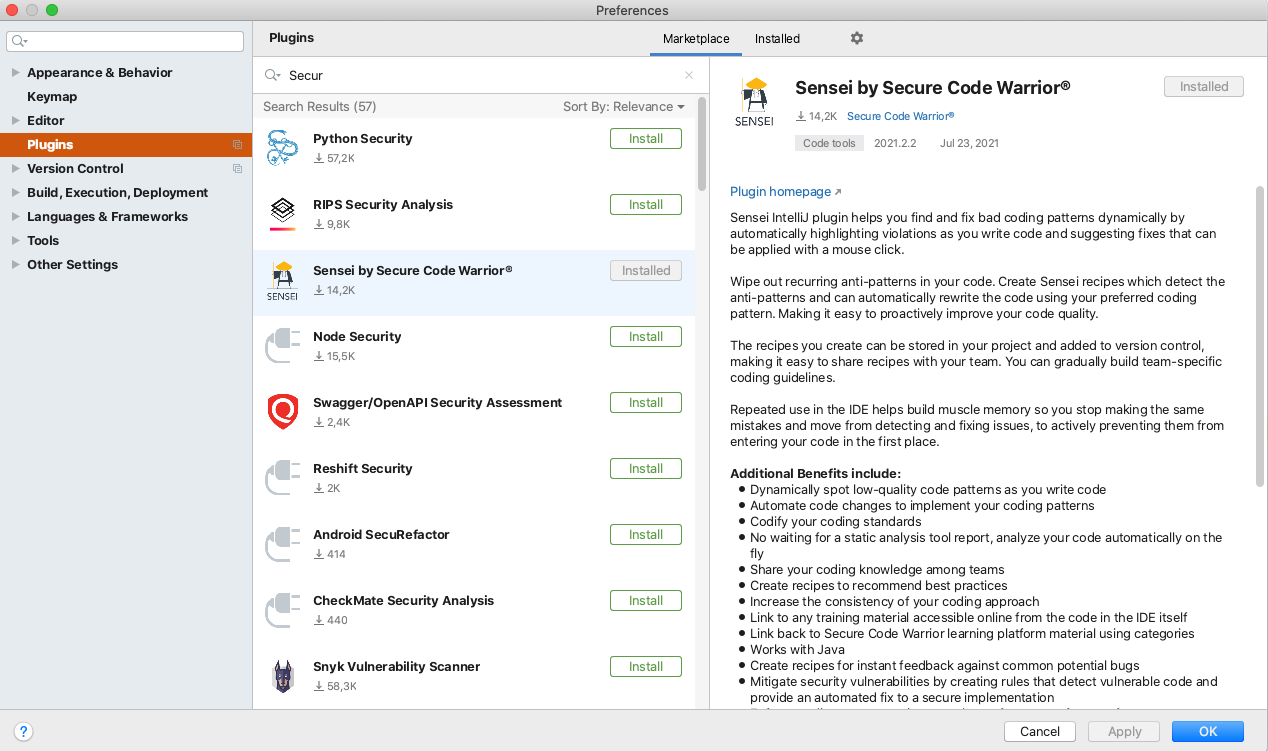
\includegraphics[width=\textwidth]{pluginsmenu.png}
  \includegraphics[width=\textwidth,page=2]{04-tools/figures/figures2.pdf}
  \caption[IntelliJ IDEA Plugins menu]{The Plugins menu in the IntelliJ IDEA allows developers to browse and easily install and uninstall extensions to their IDE.}
  \label{fig:pluginsmenu} 
\end{figure}

Sensei is available in the JetBrains Marketplace and can be installed through this Plugins menu.
Customized versions of Sensei can also be installed through this menu.
Such customized versions might be useful to disable certain features, or to automatically include certain rule sets.
To install customized versions, the Plugins menu needs to be configured to use additional plugin repositories, as shown in Figure~\ref{fig:pluginrepos}.
In this menu the developer needs to add a \gls{url} to locate the Sensei version that should be installed.
The customized version will then show up in the list of plugins in the regular menu.
This installation process is used in an experiment as described in Section~\ref{sec:experiment}.

\begin{figure}
  \centering
  %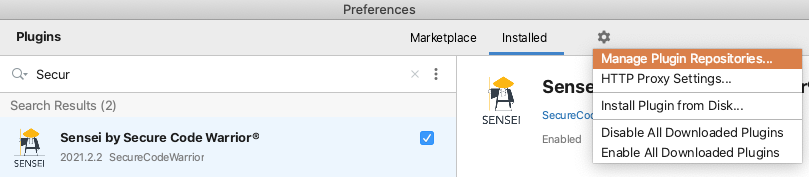
\includegraphics[width=\textwidth]{pluginrepos.png}
  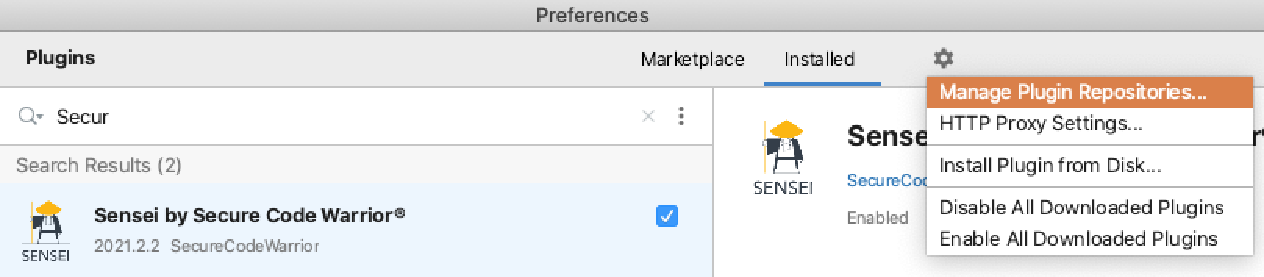
\includegraphics[width=\textwidth,page=1]{04-tools/figures/figures2.pdf}
  \caption[Adding plugin repositories to the Plugins menu]{The Plugins menu can be configured to add additional repositories of plugins, this allows us to install custom versions of the Sensei plugin that should not be distributed publicly.}
  \label{fig:pluginrepos} 
\end{figure}